%! TeX root = report.tex

\section{\SpecOne{}: Translation from Python}\label{sec:spec1}

\begin{figure}
    \centering
    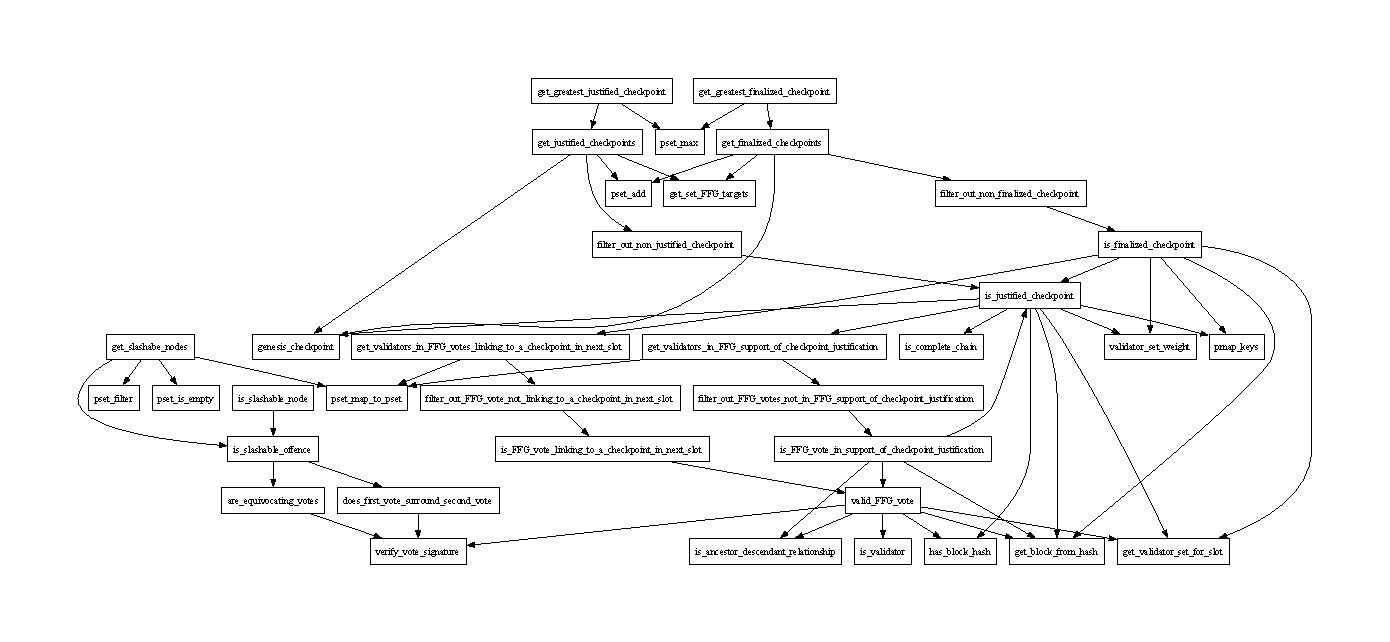
\includegraphics[width=.9\textheight,angle=-90]{ffg-callgraph.pdf}
    \caption{The callgraph of the 3SF specification}
    \label{fig:callgraph}
\end{figure}

The Python specification consists of class / type definitions and a number of
functions that define the behavior of the 3SF protocol. We obtain \SpecOne{} by
performing a manual but mechanical translation of the Python specification to
\tlap{}. To this end, we first survey the Python code to identify its structure
and the program logic elements that it defines. We then translate these
functions to \tlap{} by following the principle of least surprise: we aimed to
preserve the syntax and semantics of the Python code as closely as possible --
at this stage, without regard to model-checking efficiency. We also translate
the data structures and types used in the Python code to their \tlap{}
counterparts. To this end, we have produced detailed translation rules, which we
present in Appendix~\ref{section3}.

\subsection{Shape of the Python Specification}

A few key points to note about the Python code are as follows:

\paragraph{Data structures and types.} Type definitions come in the form of
Python classes annotated with the \texttt{@dataclass} decorator, which
automatically generates constructors, comparator methods, and other boilerplate
code. Composite types are defined using the \texttt{pyrsistent} library, which
provides immutable data structures such as sets and maps.

\paragraph{Functions.} The function definitions are mostly pure functions that
take some input and return some output -- side-effects are rare and limited to
auxiliary state when computing the function output. Some functions are
(mutually) recursive, as can be seen in Figure~\ref{fig:callgraph}.

\paragraph{Similarities between Python and \tlap{}.} Despite being a programming
language and specification language respectively, Python specifications written
in a functional manner (using immutable data types and pure functions) and
\tlap{} overlap somewhat in what they can express. For instance, both allow us
to express sets, structures / records, and comprehensions over these data
structures. For example, the Python code defines a record
\texttt{CommonNodeState} which we translate to a record in \tlap{}.

\subsection{Translating Basic Operators}

The Python specification defines a number of
foundational operators that are used in other functions. These operators are
mostly simple and can be translated directly to built-in operators in \tlap{}.
To take a concrete example, observe the definition of \texttt{pset\_filter} in
Figure~\ref{py_filter}.

\begin{figure}
  \begin{lstlisting}[language=Python,style=mystyle]
def pset_filter(p: Callable[[T1], bool], s: PSet[T1]) -> PSet[T1]:
  r: PSet[T1] = pset()
 
  for e in s:
    if p(e):
      r = r.add(e)
  
  return r\end{lstlisting}
  %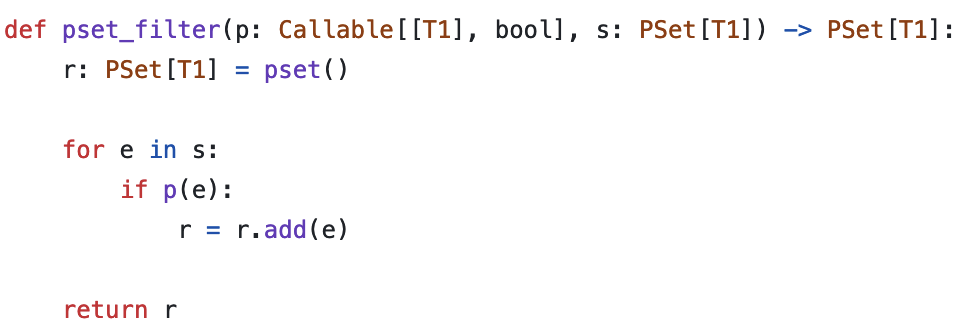
\includegraphics[width=\textwidth]{images/pset_filter.png}
\caption{\textsf{pset\_filter} definition\label{py_filter}}
\end{figure}

Notice that, while filter is not one of the built-in operators of the
\texttt{pyrsistent} library, it is relatively simple to define the
\texttt{pset\_filter} filter function, which returns a set that contains exactly
all of the elements of $s$, for which the Boolean predicate $p$ holds true.

In \tlap{}, however, filtering is a language primitive, so if we can translate a
python set $s$ to a \tlap{} set $\hat{s}$, and a Python predicate $p$ (of the
above type) to a \tlap{} predicate $\hat{p}$, we can translate
$\mathsf{pset\_filter}(p, s)$ to $\{ x \in \hat{s}\colon \hat{p}(x) \}$.

We take this idea, and apply it to every definition in the file
\texttt{pythonic\_code\_generic.py}, attempting to identify \tlap{}-equivalents
(w.r.t.\ semantics) for each defined function.  Later on, in
Appendix~\ref{section3}, we give a formal characterization of all of these
equivalencies, in the form of rewriting rules.

\subsection{Translating Complex Operators}

Some further constructs of the Python language are particularly
relevant for the translation, and we describe how we handle them in the next
paragraphs. We do, however, not give explicit rules for the translation of
\emph{all} Python language primitives to \tlap{} in general, since attempting to
establish those for the full language would vastly exceed the scope of this
project.

\paragraph{Assignments and local variables.} There are certain idiosyncrasies to
do with the fact that Python is imperative and executable, and \tlap{} is not.
For instance, Python allows for arbitrary variable assignment and reassignment,
as well as the introduction of local variables. There are two constructs
available in \tlap{} which can be used to express variable assignment:
\begin{itemize}
  \item a state-variable update $a' = e$
  \item a LET-IN local operator definition $\mathrm{LET}\; v \defeq e
    \;\mathrm{IN}\; f$
\end{itemize}

In principle, it is up to the translator to evaluate which of the two better
captures the semantics of the Python code. However, as we have noted, the Python
code is mostly functional over immutable data structures. In this project, we
have observed that we can establish a clear separation, which always translates
local/auxiliary variables to LET-IN definitions, and keeps the state-variable
updates for the state of the system.

\paragraph{Runtime exceptions.} Python code may throw at any time.
In this project in particular, the Python code is written in a defensive
manner, with many runtime checks in the form of \texttt{Requires} assertions
that perform as preconditions. 
In general, this behavior is impossible to replicate without very convoluted
\tlap{} code, so we either have to omit those assertions, or return an
unspecified value of the correct type if the requirement is not met.
We note, however, that in the present Python specification, functions are only
called if their preconditions are met (for example, the function
\texttt{get\_parent(block, node\_state)} contains a precondition
\texttt{Requires(has\_parent(block, node\_state))}, but is only ever called on
code paths where this precondition holds). Thus, we can safely omit these
assertions in the translation.

\paragraph{Control flow.} Given the functional nature of the Python
specification, and given that both languages support if-statements, those
translate directly (although since \texttt{elif} in Python has no direct
equivalent, we have to chain two IF-ELSEs in \tlap{}). Iteration (in the form of
\texttt{for}-\texttt{in} loops) only occurs in the Python code to compute the set
comprehension \texttt{pset\_filter} which we directly translate to the \tlap{}
set comprehension operator as discussed above.

\paragraph{Recursion.} As we have mentioned, the Python code contains a number
of (mutually) recursive functions. Native \tlap{} supports recursive operators
at the language level, which must be explicitly annotated with the keyword
\texttt{RECURSIVE}, which we introduce manually.

However, Apalache does not support recursive \tlap{} operators at the
model-checking level. This means that we can translate recursive Python
functions -- as written -- into \tlap{} \SpecOne{}, with the knowledge that we
will need to transform them into equivalent constructs in \SpecTwo{} to
facilitate model checking. We discuss this in more detail in the next section on
\SpecTwo{}.

\subsection{Overall Example}

As a final example, Figure~\ref{py_adr} shows a crucial operator of the Python
specification, \texttt{is\_ancestor\_descendant\_relationship}, and
Figure~\ref{tla_adr} shows its \tlap{} equivalent. It is a recursive function,
uses if-else control flow, and references \texttt{has\_parent} and
\texttt{get\_parent}, which are \tlap{}-translated python operators themselves. 

In summary, this example demonstrates that our translation strongly preserves
the syntactic shape between Python functions / compound statements and \tlap{}
operators.

\begin{figure}
  %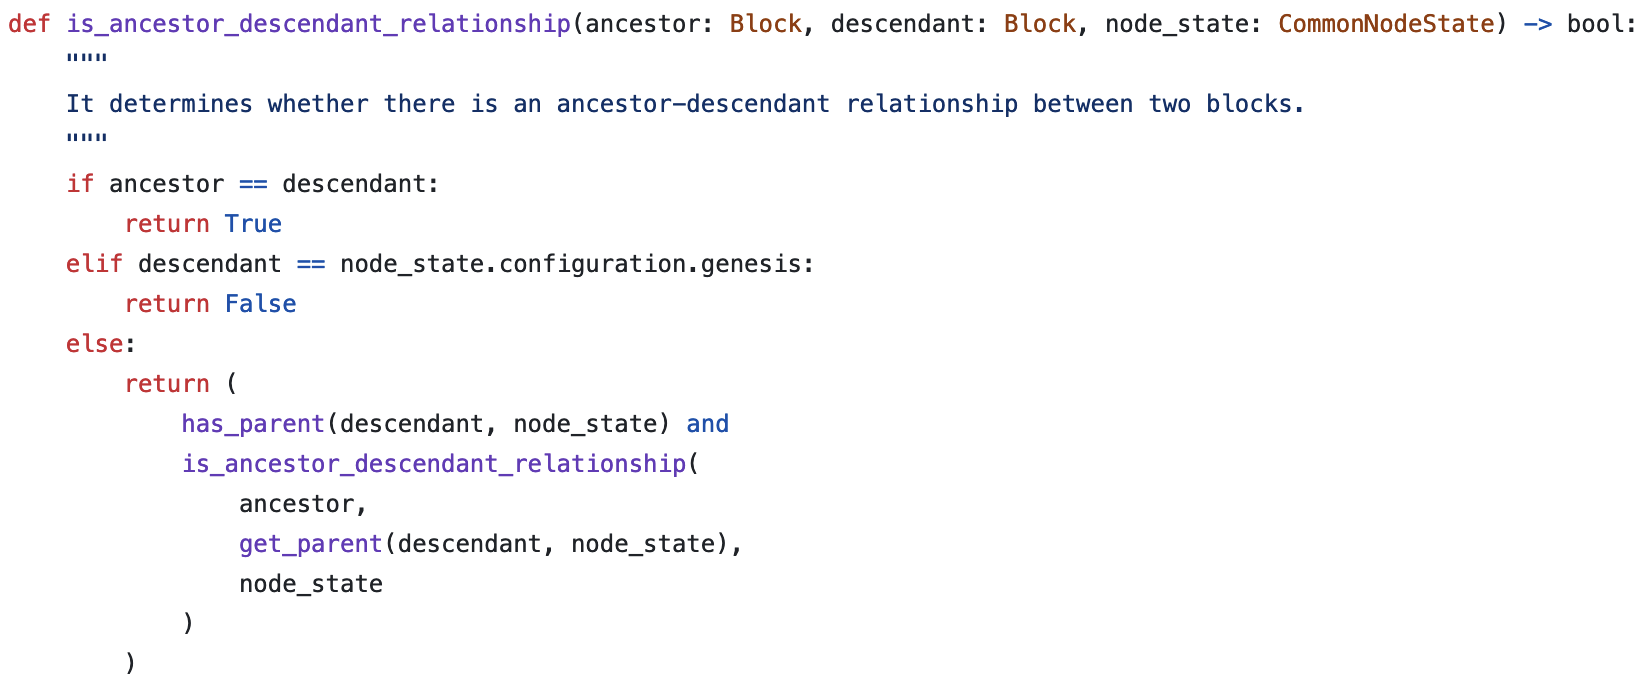
\includegraphics[width=\textwidth]{images/is_ancestor_descendant_relationship.png}

  \begin{lstlisting}[style=mystyle,language=Python]
  def is_ancestor_descendant_relationship(
    ancestor: Block, 
    descendant: Block, 
    node_state: CommonNodeState
  ) -> bool:
    """
    It determines whether there is an ancestor-descendant relationship between two blocks.
    """
    if ancestor == descendant:
        return True
    elif descendant == node_state.configuration.genesis:
        return False
    else:
        return (
            has_parent(descendant, node_state) and
            is_ancestor_descendant_relationship(
                ancestor,
                get_parent(descendant, node_state),
                node_state
            )
        )\end{lstlisting}
  \caption{Python definition
      of~\textsf{is\_ancestor\_descendant\_relationship} Python}\label{py_adr}
\end{figure}

\begin{figure}
  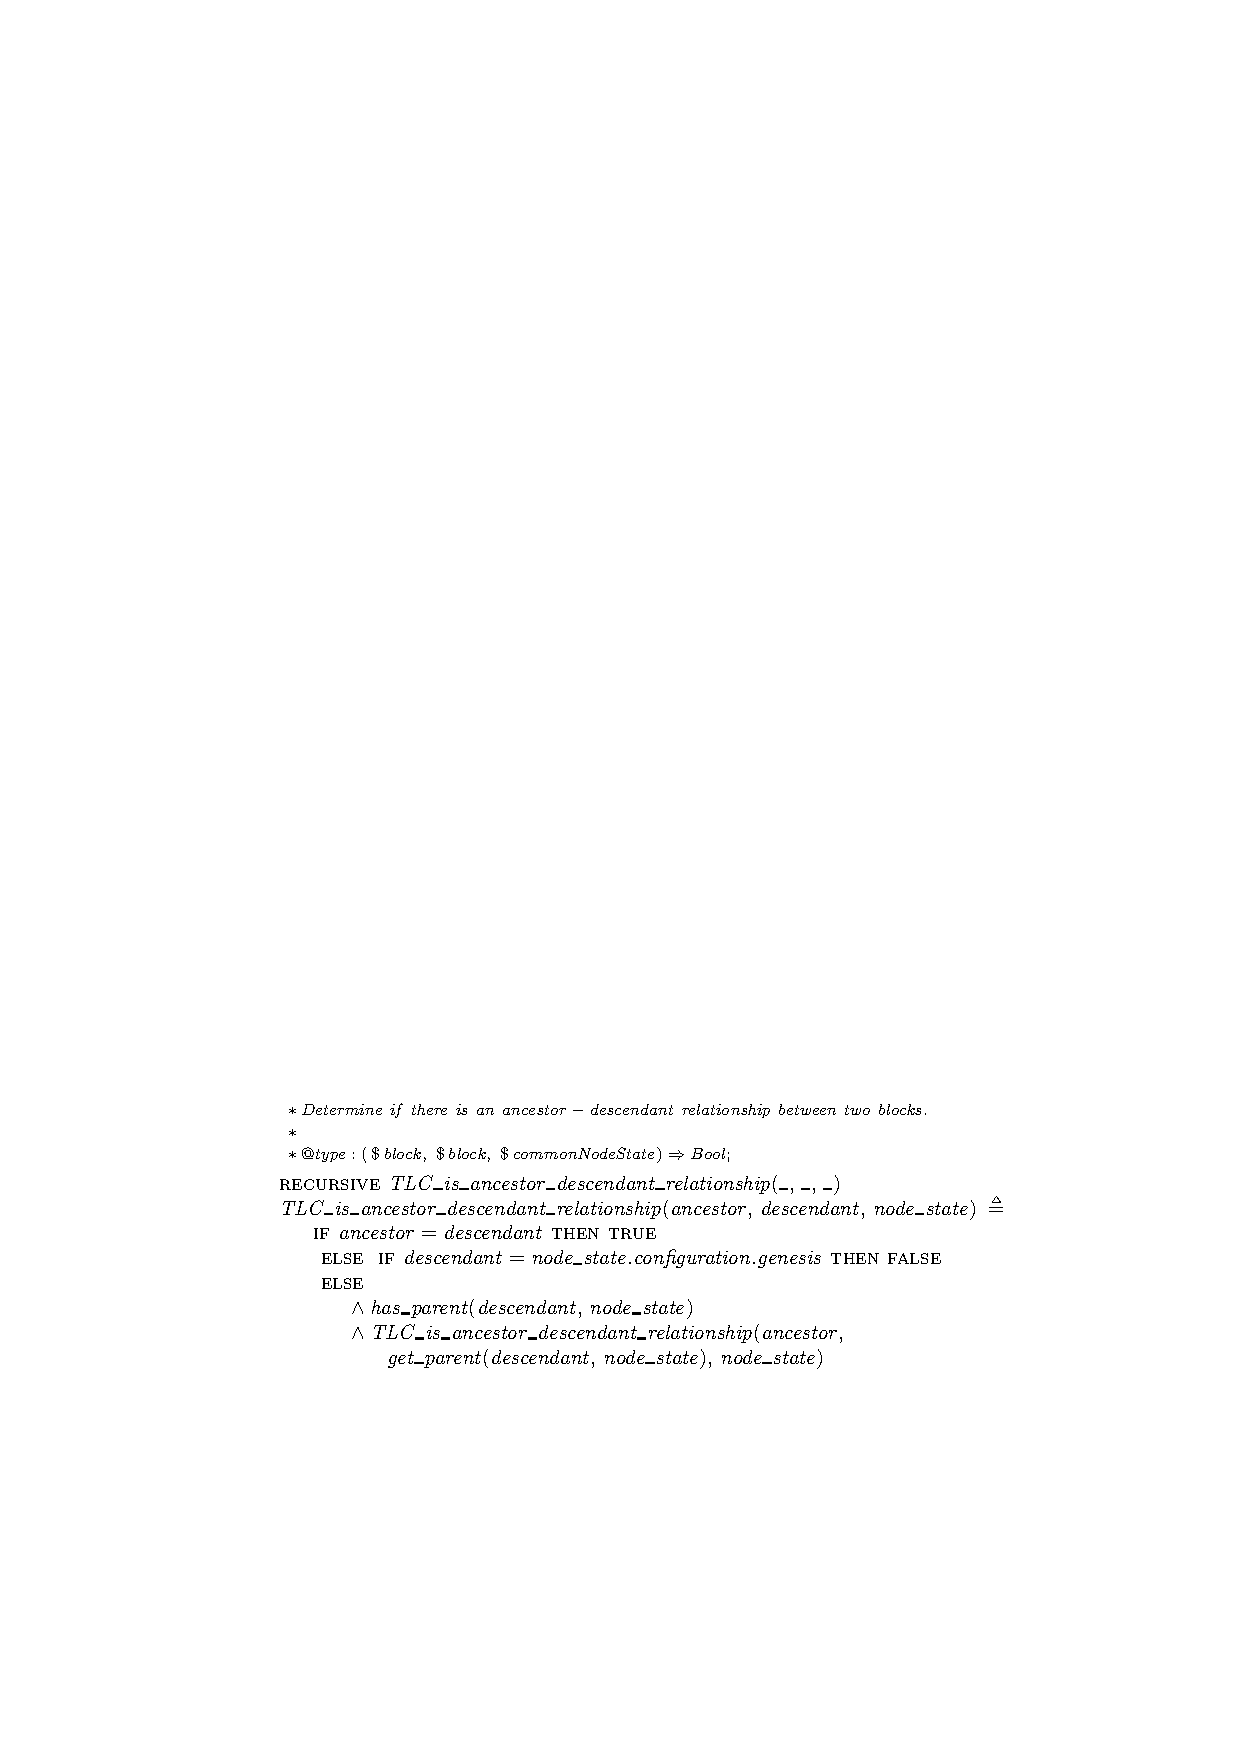
\includegraphics[width=\textwidth]{images/ancestor_descendant.pdf}
  \caption{Definition
    of~\textsf{is\_ancestor\_descendant\_relationship} in \tlap{}}\label{tla_adr}
\end{figure}

